

\documentclass[12pt]{report}
\usepackage[utf8]{inputenc}
\usepackage[russian]{babel}
\usepackage[14pt]{extsizes}
\usepackage{listings}
\usepackage{graphicx}
\usepackage{amsmath,amsfonts,amssymb,amsthm,mathtools} 
\usepackage{pgfplots}
\usepackage{filecontents}
\usepackage{float}
\usepackage{indentfirst}
\usepackage{eucal}
\usepackage{enumitem}
%s\documentclass[openany]{book}
\frenchspacing

\usepackage{titlesec}
\titleformat{\section}
{\normalsize\bfseries}
{\thesection}
{1em}{}
\titlespacing*{\chapter}{0pt}{-30pt}{8pt}
\titlespacing*{\section}{\parindent}{*4}{*4}
\titlespacing*{\subsection}{\parindent}{*4}{*4}

\usepackage{indentfirst} % Красная строка

\usetikzlibrary{datavisualization}
\usetikzlibrary{datavisualization.formats.functions}

\usepackage{amsmath}


% Для листинга кода:
\lstset{ %
	language=c,                 % выбор языка для подсветки (здесь это С)
	basicstyle=\small\sffamily, % размер и начертание шрифта для подсветки кода
	numbers=left,               % где поставить нумерацию строк (слева\справа)
	numberstyle=\tiny,           % размер шрифта для номеров строк
	stepnumber=1,                   % размер шага между двумя номерами строк
	numbersep=5pt,                % как далеко отстоят номера строк от подсвечиваемого кода
	showspaces=false,            % показывать или нет пробелы специальными отступами
	showstringspaces=false,      % показывать или нет пробелы в строках
	showtabs=false,             % показывать или нет табуляцию в строках
	frame=single,              % рисовать рамку вокруг кода
	tabsize=2,                 % размер табуляции по умолчанию равен 2 пробелам
	captionpos=t,              % позиция заголовка вверху [t] или внизу [b] 
	breaklines=true,           % автоматически переносить строки (да\нет)
	breakatwhitespace=false, % переносить строки только если есть пробел
	escapeinside={\#*}{*)}   % если нужно добавить комментарии в коде
}


\usepackage[left=2cm,right=2cm, top=2cm,bottom=2cm,bindingoffset=0cm]{geometry}
% Для измененных титулов глав:
\usepackage{titlesec, blindtext, color} % подключаем нужные пакеты
\definecolor{gray75}{gray}{0.75} % определяем цвет
\newcommand{\hsp}{\hspace{20pt}} % длина линии в 20pt
% titleformat определяет стиль
\titleformat{\chapter}[hang]{\Huge\bfseries}{\thechapter\hsp\textcolor{gray75}{|}\hsp}{0pt}{\Huge\bfseries}


% plot
\usepackage{pgfplots}
\usepackage{filecontents}
\usetikzlibrary{datavisualization}
\usetikzlibrary{datavisualization.formats.functions}

\begin{document}
	%\def\chaptername{} % убирает "Глава"
	\thispagestyle{empty}
	\begin{titlepage}
		\noindent \begin{minipage}{0.15\textwidth}
			
\includegraphics[width=\linewidth]{img/b_logo}
		\end{minipage}
		\noindent\begin{minipage}{0.9\textwidth}\centering
			\textbf{Министерство науки и высшего образования Российской Федерации}\\
			\textbf{Федеральное государственное бюджетное образовательное учреждение высшего образования}\\
			\textbf{~~~«Московский государственный технический университет имени Н.Э.~Баумана}\\
			\textbf{(национальный исследовательский университет)»}\\
			\textbf{(МГТУ им. Н.Э.~Баумана)}
		\end{minipage}
		
		\noindent\rule{18cm}{3pt}
		\newline\newline
		\noindent ФАКУЛЬТЕТ $\underline{\text{«Информатика и системы управления»}}$ \newline\newline
		\noindent КАФЕДРА $\underline{\text{«Программное обеспечение ЭВМ и информационные технологии»}}$\newline\newline\newline\newline\newline
		
		\begin{center}
			\noindent\begin{minipage}{1.1\textwidth}\centering
				\Large\textbf{  Отчет по лабораторной работе №1}\newline
				\textbf{по дисциплине <<Функциональное и логическое}\newline
				\textbf{~~~программирование>>}\newline\newline
			\end{minipage}
		\end{center}
		
		\noindent\textbf{Тема} $\underline{\text{Списки в Lispе. Использование стандартных функций.}}$\newline\newline
		\noindent\textbf{Студент} $\underline{\text{Зайцева А. А.~~~~~~~~~~~~~~~~~~~~~~~~~~~~~~~~~~~~~~~~~~}}$\newline\newline
		\noindent\textbf{Группа} $\underline{\text{ИУ7-62Б~~~~~~~~~~~~~~~~~~~~~~~~~~~~~~~~~~~~~~~~~~~~~~~~~~}}$\newline\newline
		\noindent\textbf{Оценка (баллы)} $\underline{\text{~~~~~~~~~~~~~~~~~~~~~~~~~~~~~~~~~~~~~~~~~~~~~~~~~}}$\newline\newline
		\noindent\textbf{Преподаватели} $\underline{\text{Толпинская Н.Б., Строганов Ю. В.~~~~~~~~~~~~~~~~~~~~~~~~~~~~}}$\newline\newline\newline
		
		\begin{center}
			\vfill
			Москва~---~\the\year
			~г.
		\end{center}
	\end{titlepage}
	
\chapter*{Теоретические вопросы}
	
\section*{1.	Элементы языка: определение, синтаксис, представление в памяти.}
	
Вся информация (данные и программы) в Lisp представляется в виде символьных выражений – S-выражений. 
	
По определению: S-выражение ::= <атом> | <точечная пара>.
	
Элементы языка Lisp включают в себя:
\begin{itemize}
		\item Атомы:
		\begin{itemize} 
		\item символы (идентификаторы) – синтаксически – набор литер (букв и цифр), начинающихся с буквы;
		\item специальные символы – {T, Nil} (используются для обозначения логических констант);
		\item самоопределимые атомы – натуральные числа, дробные числа, вещественные числа, строки – последовательность символов, заключенных в двойные апострофы (например, “abc”);
		\end{itemize} 
		
		\item Более сложные данные – списки и точечные пары (структуры), которые строятся с помощью унифицированных структур – блоков памяти – бинарных узлов.
		Определения:
		
		Точечная пара ::= (<атом> . <атом>) | (<атом> . <точечная пара>) | (<точечная пара> . <атом>) | (<точечная пара> . <точечная пара>);
		
		Список ::= <пустой список> | <непустой список>, где 
		
		<пустой список> ::= () | Nil,
		
		<непустой список> ::= (<первый элемент> . <хвост>),
		
		<первый элемент> ::= <S-выражение>,
		
		<хвост> ::= <список>.
		
		Список – это частный случай S-выражения.
		
\end{itemize}

Синтаксически:

любая структура (точечная пара или список) заключается в круглые скобки: (A . B) – точечная пара, (A) – список из одного элемента. Пустой список изображается как Nil или ();

непустой список по определению может быть изображен: (A . (B . (C . (D . ())))),  допустимо изображение списка последовательностью атомов, разделенных пробелами – (A B C D).

Элементы списка могут быть списками (любой список заключается в круглые скобки), например – (A (B C) (D С)). Таким образом, синтаксически наличие скобок является признаком структуры – списка или точечной пары.

Любая непустая структура Lisp в памяти представляется списковой ячейкой, хранящей два указателя: на голову (первый элемент) и хвост – всё остальное. Точечная пара в памяти представляется бинарным узлом.

\section*{2.	Особенности языка Lisp. Структура программы. Символ апостроф.}

Отличительные особенности Lisp: только символьная обработка; все можно представить в виде функций.
	
Вся информация (данные и программы) в Lisp представляется в виде символьных выражений – S-выражений. 

По определению: S-выражение ::= <атом> | <точечная пара>.
	
В зависимости от контекста одни и те же объекты могут играть роль переменных или констант, причем значения и того, и другого могут быть произвольной сложности. Если объект играет роль константы, то для объявления константы достаточно заблокировать его вычисление, то есть как бы взять его в кавычки, отмечающие буквально используемые фразы, не требующие обработки. 

Апостроф – сокращённое обозначение функции quote.

quote - блокирует вычисление своего аргумента. В качестве своего значения выдаёт сам аргумент, не вычисляя его. Перед константами - числами и атомами T, Nil можно не ставить апостроф.




\section*{3.	Базис языка Lisp. Ядро языка.}
Базис -- это минимальный набор инструментов языка и стркутур данных, который позволяет решить любые задачи.


Базис Lisp :

\begin{itemize}
	\item атомы и структуры (представляющиеся бинарными узлами);
	\item базовые (несколько) функций и функционалов: встроенные — примитивные 
	функции (atom, eq, cons, car, cdr); специальные функции и функционалы (quote, 
	cond, lambda, eval, apply, funcall).

\end{itemize}
	
Функцией называется правило, по которому каждому значению одного или нескольких  аргументов ставится в соответствие конкретное значение результата.

Функционалом, или функцией высшего порядка называется функция, аргументом или  результатом которой является другая функция.

Некоторые функции системы необходимо реализовывать в виде машинных подпрограмм, они образуют ядро системы. Ядро - основные действия, которые наиболее часто используются. Понятие <<ядро>> шире, чем понятие <<базис>>.

	
\chapter*{Практические задания}	

\section*{1. Представить следующие списки в виде списочных ячеек}

1. '(open close halph)

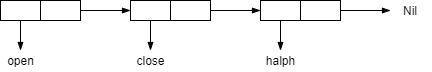
\includegraphics[scale=1]{img/1.1}

2. '((open1) (close2) (halph3))

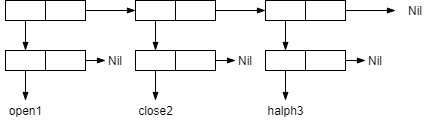
\includegraphics[scale=1]{img/1.2}

3. '((one) for all (and (me (for you))))

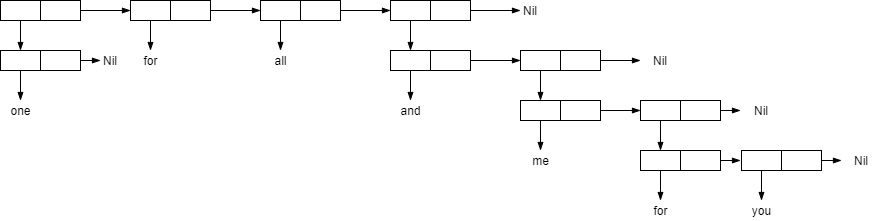
\includegraphics[scale=0.6]{img/1.3}

4. '((TOOL) (call))

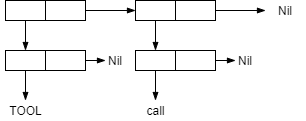
\includegraphics[scale=1]{img/1.4}

\clearpage
5. '((TOOL1) ((call2)) ((sell)))

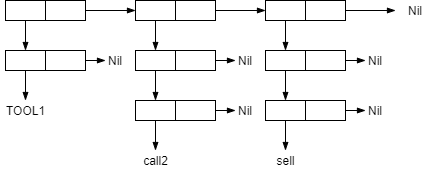
\includegraphics[scale=1]{img/1.5}

6. '(((TOOL) (call)) ((sell)))

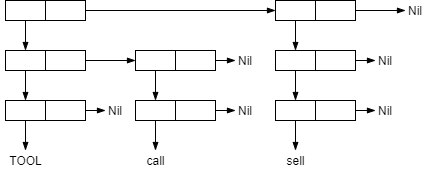
\includegraphics[scale=1]{img/1.6}


\section*{2. Используя только функции CAR и CDR, написать выражения, возввращающие:}

1. второй

\begin{lstlisting}[language=Lisp]
	(CAR (CDR '(1 2 3 4 5))) => 2
	
	(CADR '(1 2 3 4 5)) => 2
\end{lstlisting}

2. третий

\begin{lstlisting}[language=Lisp]
	(CAR (CDR (CDR '(1 2 3 4 5)))) => 3
	
	(CADDR '(1 2 3 4 5)) => 3
\end{lstlisting}

3. четвертый элементы заданного списка

\begin{lstlisting}[language=Lisp]
	(CAR (CDR (CDR (CDR '(1 2 3 4 5))))) => 4
	
	(CADDDR '(1 2 3 4 5)) => 4
\end{lstlisting}

\section*{3. Что будет в результате вычисления выражений?}

1. (CAADR '((blue cube) (red pyramid)))

\begin{lstlisting}[language=Lisp]
	(CAADR '((blue cube) (red pyramid))) => red
	1. (CDR '((blue cube) (red pyramid))) => ((red pyramid))
	2. (CAR '((red pyramid))) => (red pyramid)
	3. (CAR '(red pyramid)) => red
\end{lstlisting}

2. (CDAR '((abc) (def) (ghi))

\begin{lstlisting}[language=Lisp]
	(CDAR '((abc) (def) (ghi))) => Nil
	1. (CAR '((abc) (def) (ghi))) => (abc)
	2. (CDR '(abc)) => Nil
\end{lstlisting}

3. (CADR '((abc) (def) (ghi)))

\begin{lstlisting}[language=Lisp]
	(CADR '((abc) (def) (ghi))) => (def)
	1. (CDR '((abc) (def) (ghi))) => ((def) (ghi))
	2. (CAR '((def) (ghi))) => (def)
\end{lstlisting}


4. (CADDR '((abc) (def) (ghi)))

\begin{lstlisting}[language=Lisp]
	(CADDR '((abc) (def) (ghi))) => (ghi)
	1. (CDR '((abc) (def) (ghi))) => ((def) (ghi))
	2. (CDR '((def) (ghi))) => ((ghi))
	3. (CAR '((ghi))) => (ghi)
\end{lstlisting}


\section*{4. Напишите результат вычисления выражений и объясните, как он получен}

quote - блокирует вычисление своего аргумента. В качестве своего значения выдаёт сам аргумент, не вычисляя его. Перед константами - числами и атомами T, Nil можно не ставить апостроф. Апостроф – сокращённое обозначение функции quote.

list - не имеет фиксированного количества аргументов. Создает и возвращает список, у которого голова - это первый аргумент, хвост - все остальные аргументы.


cons - имеет фиксированное количество аргументов (два). В случае, когда аргументами являются атомы создает точечную пару. В случае, когда первый аргумент -- атом, а второй -- список, атом становится головой, а второй аргумент (список) становится хвостом. Если второе значение не NIL и не другая cons-ячейка, то ячейка печатается как два значения в скобках, разделённые точкой (так называемая точечная пара).

	
\clearpage

\begin{lstlisting}[language=Lisp]

	(list 'Fred 'and 'Wilma) => (Fred and Wilma). 
	(list 'Fred '(and Wilma)) => (Fred (and Wilma))
	(cons Nil Nil) => (Nil . Nil) => (Nil)
	(cons T Nil) => (T . Nil) => (T)
	(cons Nil T) => (Nil . T)
	(list Nil) => (Nil)
	(cons '(T) Nil)	 => ((T) . Nil)	 => ((T))
	(list '(one two) '(free temp)) => ((one two) (free temp))
	
	(cons 'Fred '(and Willma)) => (Fred . (and Willma)) => (Fred and Willma)
	(cons 'Fred '(Wilma)) => (Fred .  (Willma)) => (Fred Willma)
	(list Nil Nil) => (Nil Nil)
	(list T Nil) => (T Nil)
	(list Nil T) => (Nil T)
	(cons T (list Nil)) => (cons T '(Nil)) => (T . (Nil)) => (T Nil)
	(list '(T) Nil) => ((T) Nil)
	(cons '(one two) '(free temp)) => ((one two) . (free temp))  => ((one two) free temp)
\end{lstlisting}

\section*{5. Написать лямбда-выражение и соответствующую функцию. Представить результаты в виде списочных ячеек.}


1. Написать функцию (f ar1 ar2 ar3 ar4), возвращающую список: ((ar1 ar2) (ar3 ar4)).
\begin{lstlisting}[language=Lisp]
	;; 
	(defun f1 (ar1 ar2 ar3 ar4) (list (list ar1 ar2) (list ar3 ar4)))
	(f1 1 2 3 4) => ((1 2) (3 4))
	;; 
	(lambda (ar1 ar2 ar3 ar4) (list (list ar1 ar2) (list ar3 ar4)))
	((lambda (ar1 ar2 ar3 ar4) (list (list ar1 ar2) (list ar3 ar4))) 1 2 3 4) => ((1 2) (3 4))
\end{lstlisting}

%

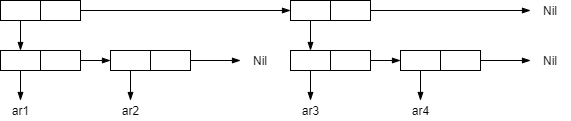
\includegraphics[scale=0.7]{img/1}

\clearpage
2. Написать функцию (f ar1 ar2), возвращающую ((ar1) (ar2)).
\begin{lstlisting}[language=Lisp]
	;;
	(defun f2 (ar1 ar2) (list (list ar1) (list ar2)))
	(f2 1 2) => ((1) (2))
	;;
	(lambda (ar1 ar2) (list (list ar1) (list ar2)))
	((lambda (ar1 ar2) (list (list ar1) (list ar2))) 1 2) => ((1) (2))
\end{lstlisting}

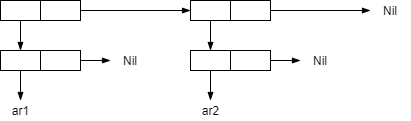
\includegraphics[scale=0.7]{img/2}


3. Написать функцию (f ar1), возвращающую (((ar1))).
\begin{lstlisting}[language=Lisp]
	;;
	(defun f3 (ar1) (list (list (list ar1))))
	(f3 1) => (((1)))
	;;
	(lambda (ar1) (list (list (list ar1))))
	((lambda (ar1) (list (list (list ar1)))) 1) => (((1)))
\end{lstlisting}

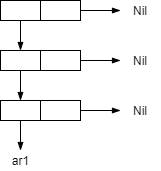
\includegraphics[scale=0.7]{img/3}

	\bibliographystyle{utf8gost705u}  % стилевой файл для оформления по ГОСТу
	
	\bibliography{51-biblio}          % имя библиографической базы (bib-файла)
	
	
\end{document}
